% COSC 3P98 Project
% gl-billiards
% Dan Lapp
% Taras Mychaskiw

\section{Controls}
Refer to Figure \ref{fig:controls} for a view of the gl-billiards window. In the figure, the user interface components are labelled.
Below is the description of each of the labelled controls.

\begin{enumerate}
    \item Informational text area. This will contain information about balls pocketed, fouls, scratches, whose turn it is
    and which ball type (solids or stripes) they are shooting for etc.
    
    \item Cue rotation. Click the double arrow and drag  the mouse left or right to rotate the cue during your shot.

    \item Shot power and control. Adjust the power of your shot by clicking the up or down arrows. You can also manually enter
    a shot power in the input (shot powers are between $0$ and $1$. Click the Shoot button to take the shot at the current angle and power selected.
    
    \item Camera rotation. Click the cross and drag the mouse in any direction to rotate the entire scene.
    
    \item Pick the center of the camera's rotation. If "Follow Ball", the camera will rotate around the ball selected in item \ref{item:follow}.
    The camera will also follow the ball as it moves around the table during a shot. If "Center of Table", the camera will rotate around the center
    of the table, and will not move as the balls are moving around the table.   \label{item:camera_center}
    
    \item Resets the camera's rotation to the default.
    
    \item Choose which ball to follow. If "Follow Ball" is selected in item \ref{item:camera_center}, then the camera will follow the selected
    ball around the table as it moves. The center of the camera's rotation will also be the selected ball here. \label{item:follow}
    
    \item Camera zoom controls. Self explanatory.
    
\end{enumerate}

Additionally, during a time when the player is allowed to move the cue ball freely, the arrow keys will move the cue ball around.
You may need to click the graphics window (the pool table area) first.

\begin{center}
    \begin{figure}[H]
        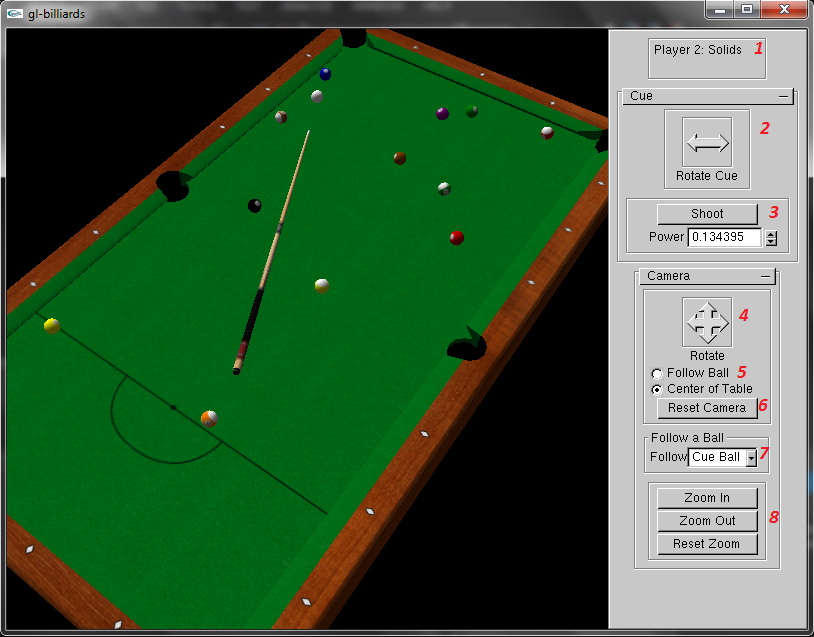
\includegraphics[scale=0.75]{controls.png}
        \caption{The gl-billiards window. Described above is what each of the controls labelled by red numbers do.}
        \label{fig:controls}
    \end{figure}
\end{center}

%\end{Controls}
